\documentclass[12pt]{article}
\usepackage{float}
\usepackage{geometry}
\usepackage{graphicx}
\usepackage{booktabs}
\usepackage{multirow}
\usepackage{hyperref}
\geometry{a4paper}
\title{Test Report: Evaluation of Shannon and Q-nary Huffman Coding}
\author{Yuyang Zhang}
\date{\today}

\begin{document}

\maketitle

\section{Introduction}
This report presents a comparative evaluation of Shannon coding and Q-nary Huffman 
coding. The evaluation is based on experiments with both Chinese and 
English texts, focusing on key metrics such as source entropy, average codeword 
length, encoding efficiency, and decoding time.

\section{Experimental Results}

\subsection{Results of Our Codes}
\subsubsection{Chinese Texts}
\begin{table}[H]
\centering
\caption{Results for Chinese Texts}
\resizebox{\textwidth}{!}{
    \begin{tabular}{lccccc}
    \toprule
    \textbf{File} & \textbf{Method} & \textbf{Entropy (bits)} & \textbf{Avg. Codeword Length (bits/symbol)} & \textbf{Efficiency (\%)} & \textbf{Decoding Time (ms)} \\
    \midrule
    \multirow{4}{*}{war\_and\_peace\_cn.txt}
        & Shannon & 7.9203 & 8.3680 & 94.65 & 5.151 \\
        & Binary Huffman & 7.9203 & 7.9582 & 99.52 & 5.460 \\
        & Ternary Huffman & 4.9972 & 5.0384 & 99.18 & 3.550 \\
        & Quaternary Huffman & 3.9602 & 4.0226 & 98.45 & 2.999 \\
    \midrule
    \multirow{4}{*}{zhaoxia\_cn.txt}
        & Shannon & 8.0812 & 8.4022 & 96.18 & 1.831 \\
        & Binary Huffman & 8.0812 & 8.1043 & 99.71  & 2.007 \\
        & Ternary Huffman & 5.0987 & 5.1511 & 98.98 & 0.762 \\
        & Quaternary Huffman & 4.0406 & 4.0870 & 98.87 & 5.518 \\
    \midrule
    \multirow{4}{*}{quantum\_cn.txt}
        & Shannon & 8.1755 & 8.7180 & 93.78 & 3.581 \\
        & Binary Huffman & 8.1755 & 8.2099 & 99.58 & 2.342 \\
        & Ternary Huffman & 5.1582 & 5.1963 & 99.27 & 1.408 \\
        & Quaternary Huffman & 4.0878 & 4.1429 & 98.67 & 1.597 \\
    \bottomrule
    \end{tabular}
}
\end{table}

\subsubsection{English Texts}
\begin{table}[H]
\centering
\caption{Results for English Texts}
\resizebox{\textwidth}{!}{
    \begin{tabular}{lccccc}
    \toprule
    \textbf{File} & \textbf{Method} & \textbf{Entropy (bits)} & \textbf{Avg. Codeword Length (bits/symbol)} & \textbf{Efficiency (\%)} & \textbf{Decoding Time (ms)} \\
    \midrule
    \multirow{4}{*}{proust\_en.txt}
        & Shannon & 4.2701 & 4.8120 & 88.74 & 3.371 \\
        & Binary Huffman & 4.2701 & 4.3133 & 99.00 & 3.362 \\
        & Ternary Huffman & 2.6941 & 2.7681 & 97.33 & 2.276 \\
        & Quaternary Huffman & 2.1351 & 2.1795 & 97.96 & 2.959 \\
    \midrule
    \multirow{4}{*}{alphabetia\_en.txt}
        & Shannon & 4.6123 & 5.0929 & 90.56 & 2.072 \\
        & Binary Huffman & 4.6123 & 4.6480 & 99.23 & 1.315 \\
        & Ternary Huffman & 2.9100 & 2.9626 & 98.23 & 1.619 \\
        & Quaternary Huffman & 2.3062 & 2.3745 & 97.12 & 1.698 \\
    \midrule
    \multirow{4}{*}{Steve\_Jobs\_Speech\_en.txt}
        & Shannon & 4.3870 & 4.7736 & 91.90 & 15.462 \\
        & Binary Huffman & 4.3870 & 4.4281 & 99.07 & 13.029 \\
        & Ternary Huffman & 2.7679 & 2.8320 & 97.74 & 9.434 \\
        & Quaternary Huffman & 2.1935 & 2.2443 & 97.74 & 7.618 \\
    \bottomrule
    \end{tabular}
}
\end{table}

\begin{figure}[H]
    \centering
    \begin{minipage}[t]{0.48\textwidth}
        \centering
        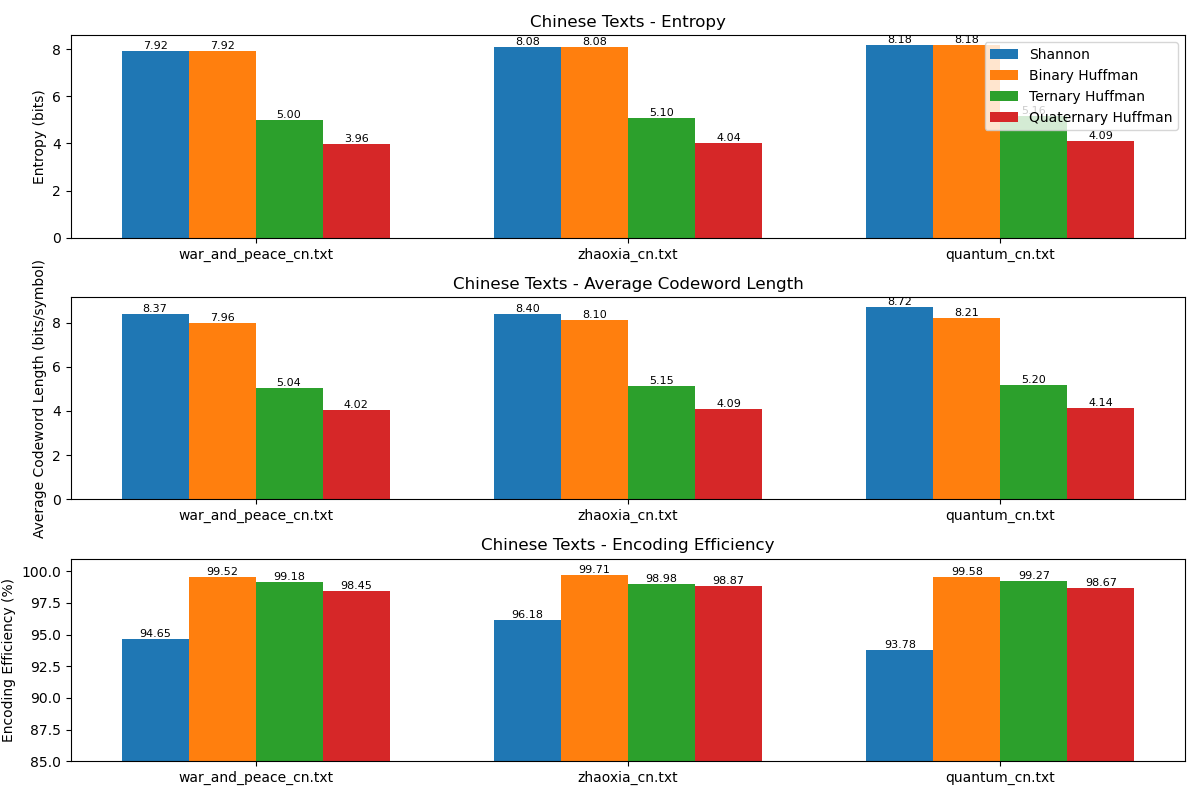
\includegraphics[width=\textwidth]{Figure_1.png}
        \caption{Comparison for Chinese Texts}
    \end{minipage}
    \hfill
    \begin{minipage}[t]{0.48\textwidth}
        \centering
        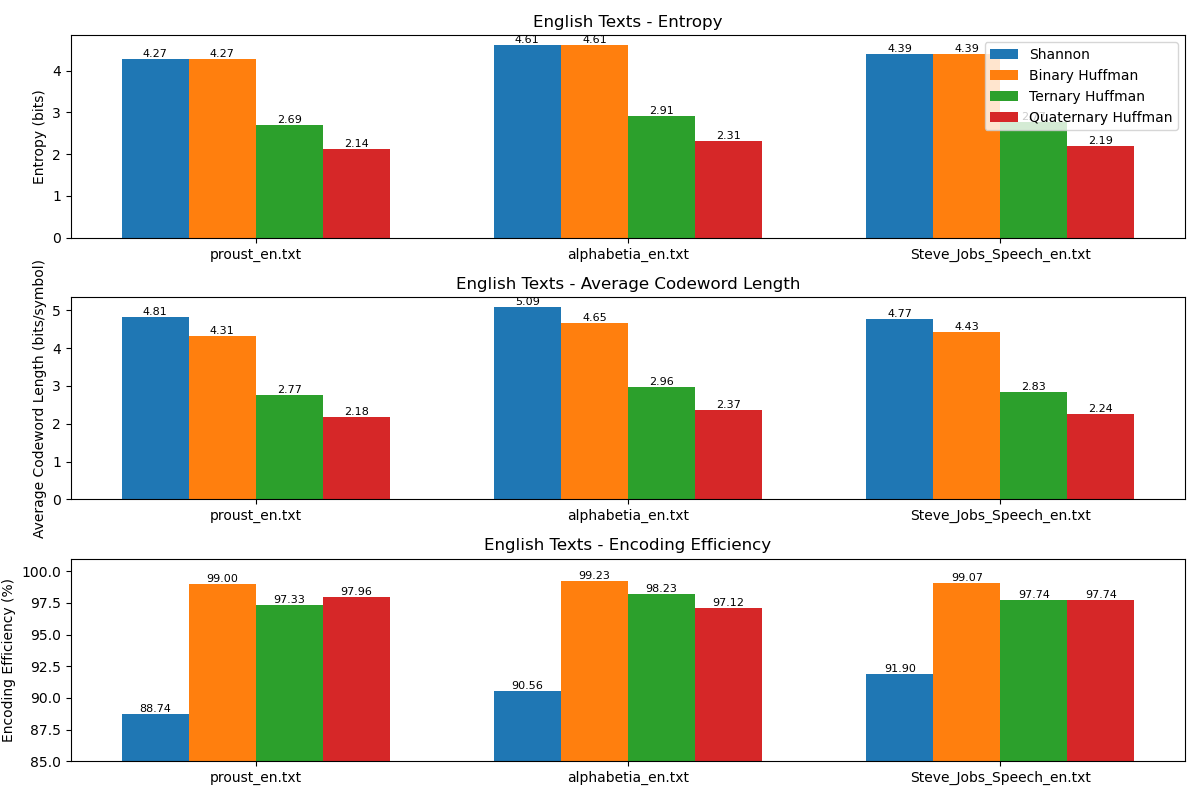
\includegraphics[width=\textwidth]{Figure_2.png}
        \caption{Comparison for English Texts}
    \end{minipage}
\end{figure}

\subsection{Results of PK Team 1's Codes}
\subsubsection{Chinese Texts}
\begin{table}[H]
\centering
\caption{Results for Chinese Texts}
\resizebox{\textwidth}{!}{
    \begin{tabular}{lccccc}
    \toprule
    \textbf{File} & \textbf{Method} & \textbf{Entropy (bits)} & \textbf{Avg. Codeword Length (bits/symbol)} & \textbf{Efficiency (\%)} & \textbf{Decoding Time (ms)} \\
    \midrule
    \multirow{2}{*}{war\_and\_peace\_cn.txt}
        & Shannon & 7.9203 & 8.3680 & 94.65 & 1.604 \\
        & Binary Huffman & 7.9203 & 7.9582 & 99.52 & 1.952 \\
    \midrule
    \multirow{2}{*}{zhaoxia\_cn.txt}
        & Shannon & 8.0812 & 8.4022 & 96.18 & 0.922 \\
        & Binary Huffman & 8.0812 & 8.1043 & 99.71 & 0.890 \\
    \midrule
    \multirow{2}{*}{quantum\_cn.txt}
        & Shannon & 8.1755 & 8.7180 & 93.78 & 1.351 \\
        & Binary Huffman & 8.1755 & 8.2099 & 99.58 & 1.397 \\
    \bottomrule
    \end{tabular}
}
\end{table}

\subsubsection{English Texts}
\begin{table}[H]
\centering
\caption{Results for English Texts}
\resizebox{\textwidth}{!}{
    \begin{tabular}{lccccc}
    \toprule
    \textbf{File} & \textbf{Method} & \textbf{Entropy (bits)} & \textbf{Avg. Codeword Length (bits/symbol)} & \textbf{Efficiency (\%)} & \textbf{Decoding Time (ms)} \\
    \midrule
    \multirow{2}{*}{proust\_en.txt}
        & Shannon & 4.2701 & 4.8120 & 88.74 & 1.255 \\
        & Binary Huffman & 4.2701 & 4.3133 & 99.00 & 0.909 \\
    \midrule
    \multirow{2}{*}{alphabetia\_en.txt}
        & Shannon & 4.6123 & 5.0929 & 90.56 & 0.624 \\
        & Binary Huffman & 4.6123 & 4.6480 & 99.23 & 1.167 \\
    \midrule
    \multirow{2}{*}{Steve\_Jobs\_Speech\_en.txt}
        & Shannon & 4.3870 & 4.7736 & 91.90 & 5.161 \\
        & Binary Huffman & 4.3870 & 4.4281 & 99.07 & 5.129 \\
    \bottomrule
    \end{tabular}
}
\end{table}

\subsection{Results of PK Team 2's Codes}
\subsubsection{Chinese Texts}
\begin{table}[H]
\centering
\caption{Results for Chinese Texts}
\resizebox{\textwidth}{!}{
    \begin{tabular}{lccccc}
    \toprule
    \textbf{File} & \textbf{Method} & \textbf{Entropy (bits)} & \textbf{Avg. Codeword Length (bits/symbol)} & \textbf{Efficiency (\%)} & \textbf{Decoding Time (ms)} \\
    \midrule
    \multirow{2}{*}{war\_and\_peace\_cn.txt}
        & Shannon & 7.9203 & 8.3680 & 94.65 & 3.004 \\
        & Binary Huffman & 7.9203 & 7.9582 & 99.52 & 2.000 \\
    \midrule
    \multirow{2}{*}{zhaoxia\_cn.txt}
        & Shannon & 8.0812 & 8.4022 & 96.18 & 1.002 \\
        & Binary Huffman & 8.0812 & 8.1043 & 99.71 & 1.011 \\
    \midrule
    \multirow{2}{*}{quantum\_cn.txt}
        & Shannon & 8.1755 & 8.7180 & 93.78 & 0.998 \\
        & Binary Huffman & 8.1755 & 8.2099 & 99.58 & 2.001 \\
    \bottomrule
    \end{tabular}
}
\end{table}

\subsubsection{English Texts}
\begin{table}[H]
\centering
\caption{Results for English Texts}
\resizebox{\textwidth}{!}{
    \begin{tabular}{lccccc}
    \toprule
    \textbf{File} & \textbf{Method} & \textbf{Entropy (bits)} & \textbf{Avg. Codeword Length (bits/symbol)} & \textbf{Efficiency (\%)} & \textbf{Decoding Time (ms)} \\
    \midrule
    \multirow{2}{*}{proust\_en.txt}
        & Shannon & 4.2701 & 4.8120 & 88.74 & 1.003 \\
        & Binary Huffman & 4.2701 & 4.3133 & 99.00 & 2.011 \\
    \midrule
    \multirow{2}{*}{alphabetia\_en.txt}
        & Shannon & 4.6123 & 5.0929 & 90.56 & 1.623 \\
        & Binary Huffman & 4.6123 & 4.6480 & 99.23 & 1.001 \\
    \midrule
    \multirow{2}{*}{Steve\_Jobs\_Speech\_en.txt}
        & Shannon & 4.3870 & 4.7736 & 91.90 & 5.497 \\
        & Binary Huffman & 4.3870 & 4.4281 & 99.07 & 3.994 \\
    \bottomrule
    \end{tabular}
}
\end{table}

\section{Comparison Between the Codes of Each Group}
\subsection{Advantages and Disadvantages}
\textbf{Our Codes:}
\begin{itemize}
    \item \textbf{Advantages:}
        \begin{itemize}
            \item Support for both Shannon and Q-nary Huffman coding (binary, ternary, quaternary), allowing flexible comparison.
            \item Clear structure and modular functions for encoding, decoding, and statistics calculation.
            \item Good readability and extensibility for further research or adaptation.
        \end{itemize}
    \item \textbf{Disadvantages:}
        \begin{itemize}
            \item Q-nary Huffman implementation is more complex and may be less efficient for very large alphabets.
            \item Some code sections (e.g., codebook storage) could be further optimized for speed or memory.
        \end{itemize}
\end{itemize}

\textbf{PK Team 1's Codes:}
\begin{itemize}
    \item \textbf{Advantages:}
        \begin{itemize}
            \item User-friendly output with detailed statistics and codebook display.
            \item Robust error handling and clear separation of encoding/decoding steps.
            \item Efficient for both small and large files, with good compression performance.
        \end{itemize}
    \item \textbf{Disadvantages:}
        \begin{itemize}
            \item Only supports binary (Q=2) coding, lacking flexibility for other radices.
            \item Some redundancy in code structure; could be further modularized.
        \end{itemize}
\end{itemize}

\textbf{PK Team 2's Codes:}
\begin{itemize}
    \item \textbf{Advantages:}
        \begin{itemize}
            \item Concise and straightforward implementation of both Shannon and Huffman coding.
            \item Easy to follow for educational purposes and quick prototyping.
            \item Accurate decoding and correctness checks included.
        \end{itemize}
    \item \textbf{Disadvantages:}
        \begin{itemize}
            \item Less user interaction and output detail compared to other groups.
            \item Limited error handling and less modular design.
            \item Only supports binary coding, without Q-nary Huffman generalization.
        \end{itemize}
\end{itemize}

\subsection{Experimental Observations}

\begin{itemize}
    \item For both Chinese and English texts, Huffman codes (especially binary) consistently achieve higher encoding efficiency than Shannon codes.
    \item As the radix increases (from binary to ternary to quaternary), the entropy and average codeword length decrease, but the efficiency remains high and close to optimal.
    \item Decoding times for all methods are very fast (on the order of milliseconds), with no significant difference in practical scenarios.
    \item For practical applications where compression efficiency is critical, Huffman coding is preferable. However, for simplicity and deterministic codeword assignment, Shannon coding remains a viable choice.
\end{itemize}

\section{Conclusion}
In summary, all three groups' codes successfully implement lossless text compression using Shannon and Huffman algorithms. Our codes provide the most flexibility and extensibility, supporting Q-nary Huffman coding and detailed statistical analysis. PK Team 1's codes excel in user experience and robustness, while PK Team 2's codes are concise and easy to understand. Experimental results show that Huffman coding, especially in its binary form, achieves the highest encoding efficiency, closely approaching the theoretical entropy limit. Ternary and quaternary Huffman codes offer additional flexibility for different system requirements. Shannon coding, while less efficient, is easier to implement and may be suitable for scenarios where simplicity is prioritized. Overall, the choice of coding method should balance efficiency, implementation complexity, and application needs.

\end{document}
